\section{Software Realization}
\label{sec:software-realization}

\subsection{Overview}
\label{ssec:overview}

\subsection{Class Diagrams}
\label{ssec:class-diagrams}
\addtocontents{toc}{\protect\setcounter{tocdepth}{2}}

% Talk about:
% - To increase cohesion and reduce coupling the agent uses multiple controllers to handle the different aspects of the agent.
%   - The controllers are connected to an event bus, which is used to communicate between the controllers.
%   - The controllers are the interfacing layer between events and services that perform the actual computations.
% - The MessageBroker is used to send messages between agents.
%   - The incoming messages are handled and dispatched to the event bus, which then triggers the appropriate controller.
%   - The outgoing messages are sent to the MessageBroker, which then sends the message to the appropriate agent. In the Experimental setup there is a single message broker which is used by all agents. In a real world scenario each agent would have their own message broker, communicating over the network through HTTP or some other protocol.
% - The ExperimentalAgent is a subclass of the Agent, which is used to simulate the agents in the experimental setup, exposing the necessary methods to the ExperimentManager.
% - The ExperimentManager observes messages sent over the MessageBroker, and is able to send messages to the agents through the MessageBroker. This is helpful when measuring metrics and controlling the behavior of agents during the experiment.

% \comment{Zoltan}{I think this doesnt belonf here, but rather into a currently missing section between the current sections 3 and 4. In which you describe the design and implementation of your program. (The current section 3 contains some stubs that also belong into this to-be-created section)}
\comment{Zoltan}{It would be a good to add an overview diagram that shows the structure of the while program on a higher level of abstraction than individual classes.}
In this section, we present an overview and analysis of a UML Class Diagram for our proposed implementation of the ADRIAN protocol\cite{mann2023ADRIAN} which can be seen in Figures \ref{fig:uml-agent} through \ref{fig:uml-services}. At a quick glance the architecture features multiple controllers, connected through an internal event bus, and a message broker external communication. Additionally, some classes have been extended to support the experimental setup, which is further explained in Section \ref{sec:experiments}.

\begin{figure}[H]
    \centering
    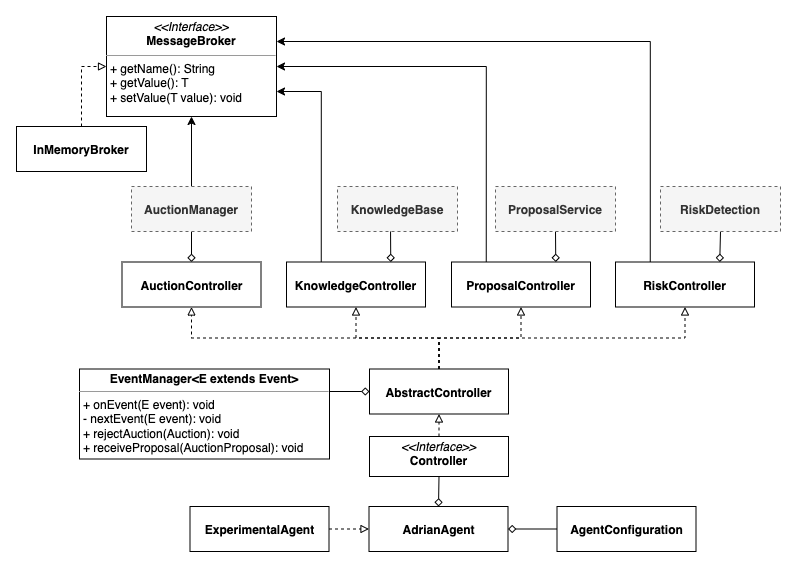
\includegraphics[width=0.8\textwidth]{_content/uml-agent}
    \caption{UML Diagram of the code structure of an Agent.}
    \label{fig:uml-agent}
\end{figure}

\subsubsection{Increased Cohesion and Reduced Coupling through Controller Interfaces}
\label{sssec:reduced-cohesion-coupling}
The systems architecture uses multiple controllers to handle various aspects of the agent, aiming to reduce both cohesion and coupling between components. Each controller is responsible for a specific set of tasks and the corresponding events, leading to a more modular and flexible design. This separation of functionality allows for easier maintenance, as well as the ability to replace controllers with new implementations, minimizing the impact on other parts of the system.
\comment{Zoltan}{Will the responsibility of each controller be described somewhere?}

\subsubsection{Event Bus for internal communication}
\label{sssec:event-bus}
To enable communication between controllers, an internal event bus is created. The event bus is in essence nothing more than a Observer pattern (also known as \texttt{EventEmitter} or \texttt{Pup/Sub}). This decouples the controllers from one another, as they are not directly aware of each other. Controllers can publish and subscribe to events on the event bus, and the event bus will then notify all subscribers when an event is published. 
\comment{Zoltan}{Should the eventbus not be visible somewhere in figure 4.}

\subsubsection{Controllers as an interfacing layer}
\label{sssec:controllers-interfacing-layer}
Controllers serve as an interfacing layer, between the event bus and the services responsible for the computations. This abstraction shields the services from the complexities of event handling, promoting modularity and reusability. It allows the services to be reused in other contexts, and makes the code easier to test as it is not dependent on any external form of communication (which is handled by the controllers).

\subsubsection{Message Broker for external communication}
\label{sssec:message-broker}
The system uses a \code{MessageBroker} which facilitates communication between agents. It allows for both incoming and outgoing messages to be handled by the agent, while abstracting away the underlying protocol. Incoming messages are processed and dispatched onto the internal event bus, triggering the relevant controllers to handle the message. On the other hand, outgoing messages are sent to the \code{MessageBroker}, which then sends the message to the appropriate agent.

The \code{MessageBroker} as an interface can be concretized by different implementations,\comment{Zoltan}{I dont understand what is meant here}depending on hardware-/software-requirements. In the experimental setup, a single \code{MessageBroker} is used by all agents and works directly in memory. This avoids any additional network complexity and allows \comment{Zoltan}{Compared to what?}a more efficient simulation. In a real world scenario, the \code{MessageBroker} would be a network service, which is used to send messages between agents over the network using HTTP requests or some other protocol such as MQTT. From the agents perspective, the \code{MessageBroker} would be the same, regardless of the implementation, and thus reducing coupling between the agents and the underlying communication protocol.

\subsubsection{Similarities in graph data structures}
\label{sssec:graph-data-structures}
In the real world the infrastructure is a graph structure, something that it \comment{Zoltan}{This could be interpreted in such a way that the speicific graph is hard-coded in the program. I think this is not what you want to say} captured in the code of the agent as well. The \code{Infrastructure}-graph consists of two types of nodes; \code{InfrastructureNode} and \code{SoftwareComponent}. These nodes can be mapped to actual hardware (e.g. Servers and IoT devices) and software (e.g. Databases and Services) in real world applications, their concrete implementation is intentionally left away in order to reduce overhead and complexity.

\begin{figure}[H]
    \centering
    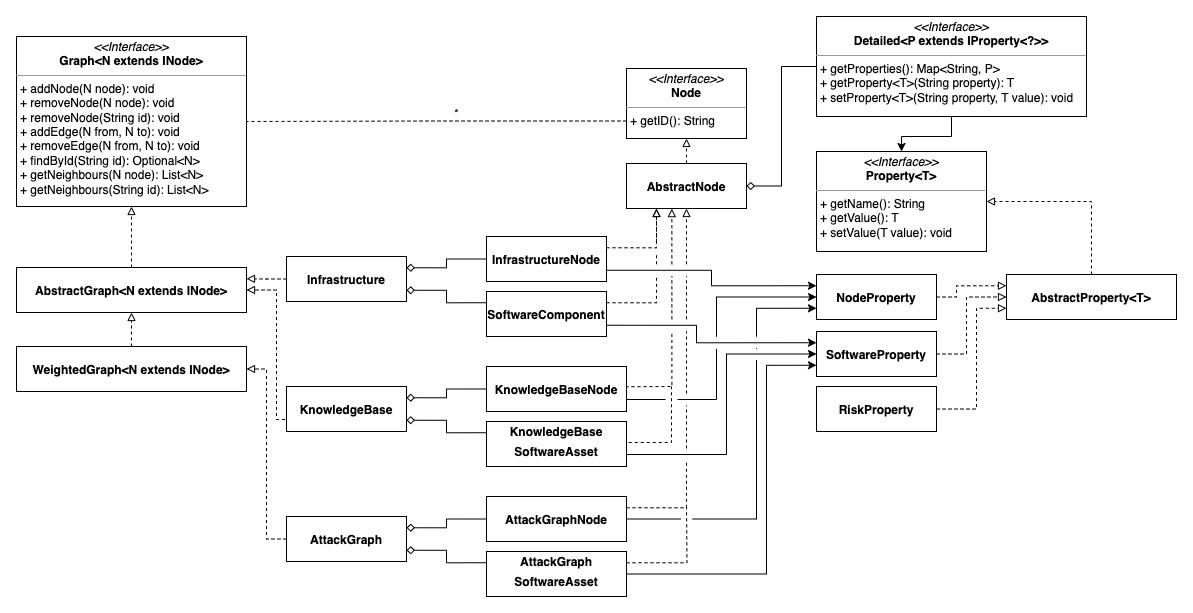
\includegraphics[width=1.2\textwidth]{_content/uml-graphs}
    \caption{UML Diagram explaining the structure of the Graphs, in a way that the separate classes are similar to their counter parts.}
    \label{fig:uml-graphs}
\end{figure}


\begin{figure}[H]
    \centering
    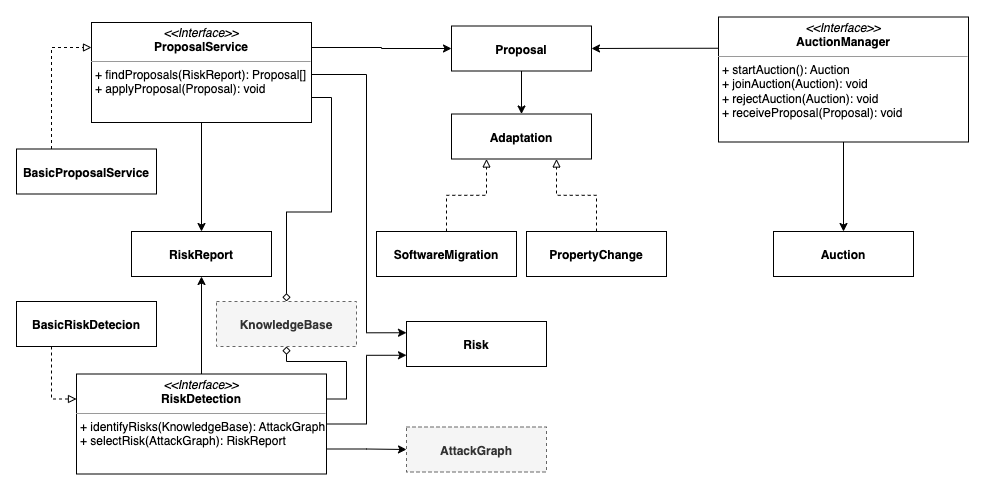
\includegraphics[width=0.8\textwidth]{_content/uml-services}
    \caption{UML Diagram depicting how the Agents services are tied together.}
    \label{fig:uml-services}
\end{figure}

\subsection{Sequence Diagrams}
\label{ssec:sequence-diagrams}
\begin{figure}[H]
    \centering
    \includegraphics[width=0.8\textwidth]{_content/knowledge-sharing}
    \caption{Knowledge Exchange Sequence Diagram}
    \label{fig:knowledge-sharing}
\end{figure}

\begin{figure}[H]
    \centering
    \includegraphics[width=0.8\textwidth]{_content/auction}
    \caption{Auction Sequence Diagram}
    \label{fig:auction}
\end{figure}

\addtocontents{toc}{\protect\setcounter{tocdepth}{3}}
